\documentclass{article}


% if you need to pass options to natbib, use, e.g.:
%     \PassOptionsToPackage{numbers, compress}{natbib}
% before loading neurips_2023


% ready for submission
\usepackage[final]{neurips_2023}


% to compile a preprint version, e.g., for submission to arXiv, add add the
% [preprint] option:
%     \usepackage[preprint]{neurips_2023}


% to compile a camera-ready version, add the [final] option, e.g.:
%     \usepackage[final]{neurips_2023}


% to avoid loading the natbib package, add option nonatbib:
%    \usepackage[nonatbib]{neurips_2023}


\usepackage[utf8]{inputenc} % allow utf-8 input
\usepackage[T1]{fontenc}    % use 8-bit T1 fonts
\usepackage{hyperref}       % hyperlinks
\usepackage{url}            % simple URL typesetting
\usepackage{booktabs}       % professional-quality tables
\usepackage{amsfonts}       % blackboard math symbols
\usepackage{nicefrac}       % compact symbols for 1/2, etc.
\usepackage{microtype}      % microtypography
\usepackage{xcolor}         % colors
\usepackage{graphicx}       % images
\usepackage{float}          % positioning
\graphicspath{ {./img/} }


\title{Proyecto Final Aprendizaje Automático}


% The \author macro works with any number of authors. There are two commands
% used to separate the names and addresses of multiple authors: \And and \AND.
%
% Using \And between authors leaves it to LaTeX to determine where to break the
% lines. Using \AND forces a line break at that point. So, if LaTeX puts 3 of 4
% authors names on the first line, and the last on the second line, try using
% \AND instead of \And before the third author name.


\author{%
    Lucía Herraiz Cano\\
    Aprendizaje Automático\\
    Universidad Pontificia Comillas\\
    Abril 2025\\
    \texttt{202300465@alu.comillas.edu} \\
}


\begin{document}


\maketitle


\begin{abstract}
  En este proyecto se desarrolla un análisis predictivo sobre el rendimiento 
  académico de estudiantes de secundaria en dos institutos de Madrid durante 
  el año 2005. A partir de un conjunto de datos, se construyen y comparan dos 
  modelos para predecir la nota final del curso (T3). También se lleva a cabo 
  un estudio de los datos y de las variables más influyentes en el desarrollo
  del estudiante. Este estudio busca no solo obtener predicciones precisas, 
  sino también generar conocimiento accionable para mejorar el rendimiento 
  estudiantil desde una perspectiva integral.
\end{abstract}


\section{Exploratory data analysis (EDA)}


En esta sección se analiza la estructura y distribución del conjunto de datos, identificando patrones, valores atípicos y relaciones relevantes entre variables. También se detalla el proceso de limpieza y preparación necesario para el modelado posterior.

El desarrollo detallado de estos análisis se encuentra principalmente documentado en \textit{Exploratory\_Data\_Analysis}. No obstante, ciertas observaciones derivadas del análisis 
conjunto con modelos predictivos pueden consultarse en \textit{Model1\_Testing} y \textit{Model2\_Testing}.


\subsection{Limpieza de datos}


El proceso de limpieza de datos viene recogido en la función \texttt{data\_cleaning\_pipeline}
e incluye el manejo de outliers, la imputación de valores faltantes, la corrección de errores, la codificación de las variables 
categóricas y la estandarización de los datos.

\begin{figure}[ht]
  \centering
  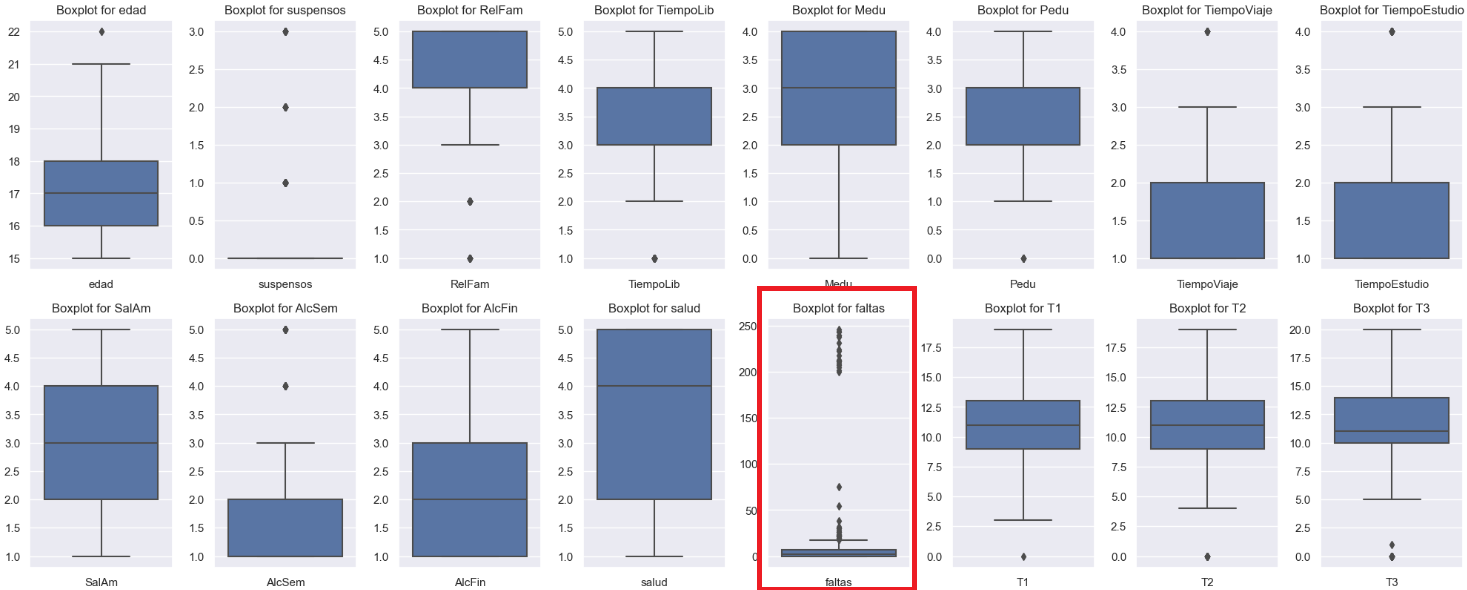
\includegraphics[width=0.7\textwidth]{Boxplot_Outliers.png}
  \caption{Boxplot de los outliers de las variables}\label{fig:boxplot}
\end{figure}

Al estudiar los outliers, la variable más llamativa fue \textit{faltas}. Se estableció un valor máximo de 150, correspondiente al número de días lectivos del calendario escolar estándar, considerando 
cualquier valor superior como erróneo. Se probaron dos estrategias adicionales, eliminar registros, e imputar los outliers por la mediana, pero ambas estrategias disminuyeron la 
\textit{performance} de los modelos en varios puntos. Esto muestra no sólo que \textit{faltas} es una variable altamente relevante, sino que en este caso los outliers son muy informativos.


Sólo 5 variables tenían valores faltantes, y con el objetivo de perder la menor cantidad de datos, todos los valores se imputaron siguiendo distintas estrategias.
\textit{AlcSem, Relfam} y \textit{TiempoEstudio} se imputaron por la moda al ser variables categóricas, y tener menos de un 3\% de valores faltantes. \textit{Medu} y \textit{Pedu}, 
al tener un porcentaje más relevante de valores faltantes, tener una correlación de Pearson alta (0.653), y al ser variables con mucho peso, como se verá posteriormente, se imputaron con un regresor (IterativeImputer) que emplea el resto de datos
para predecir sus valores de manera más robusta. 

Se corrigieron los datos de la columna \textit{razon} al tener claves distintas para el mismo valor ("otras", "otros").

Finalmente, tras estudiar el balance de las clases, se vió que \textit{EstPadres, EstSup} y \textit{apoyo} estaban claramente desbalanceadas (80\%-20\%). Sin embargo, dado que ninguna es una variable
muy relevante, y dado que los resultados reflejan bien el balance que se suele dar en la población real, se decidió mantener los datos y tener cuidado con los modelos que le den relevancia a estas variables.

Tras limpiar los datos, se hizo un \textit{dummy encoding}, en lugar de \textit{one hot encoding}, sobre las variables categóricas, para no añadir columnas innecesarias al dataset. La \textit{performance} de los modelos se vió muy beneficiada por la estandarización de las variables numéricas, lo que tiene sentido ya que los datos se interpretan por los modelos de manera similar, sin depender de su escala.
Sin embargo, es importante añadir que para evitar el \textit{data leakage}, la estandarización de los datos se llevó a cabo durante todo el proyecto tras separar los datos entre \textit{Train} y \textit{Test}, utilizando solo la información de los datos de \textit{Train}. 

\subsection{Análisis no supervisado}


Con el objetivo de comprender mejor la relevancia y relación de las variables, se implementaron técnicas de aprendizaje no supervisado. 

\begin{figure}[h!]
  \centering
  \begin{minipage}[b]{0.45\textwidth}
      \centering
      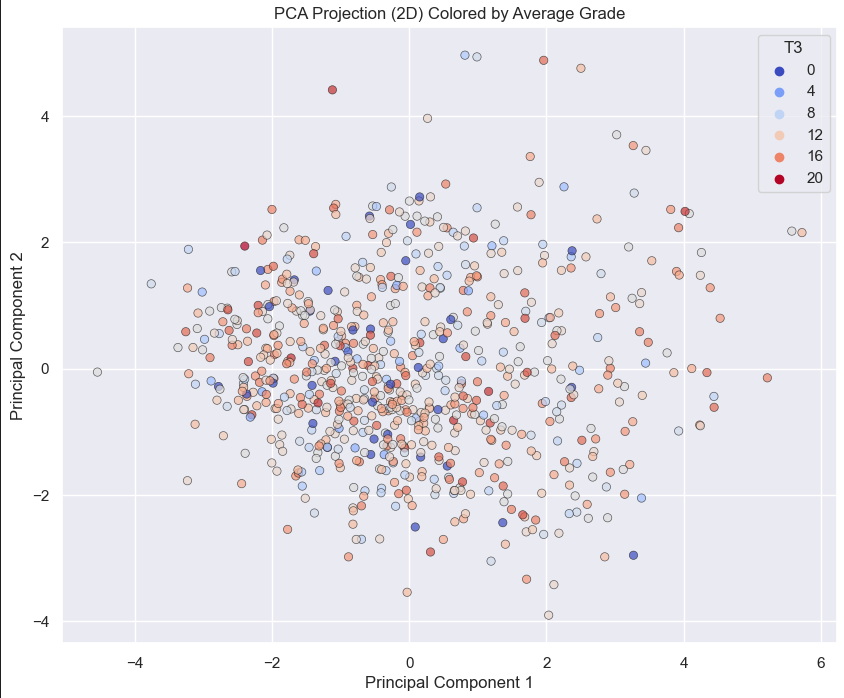
\includegraphics[scale=0.30]{PCA2PC.png}
      \caption{(a) PCA con 2 PC}
  \end{minipage}
  \hfill
  \begin{minipage}[b]{0.45\textwidth}
      \centering
      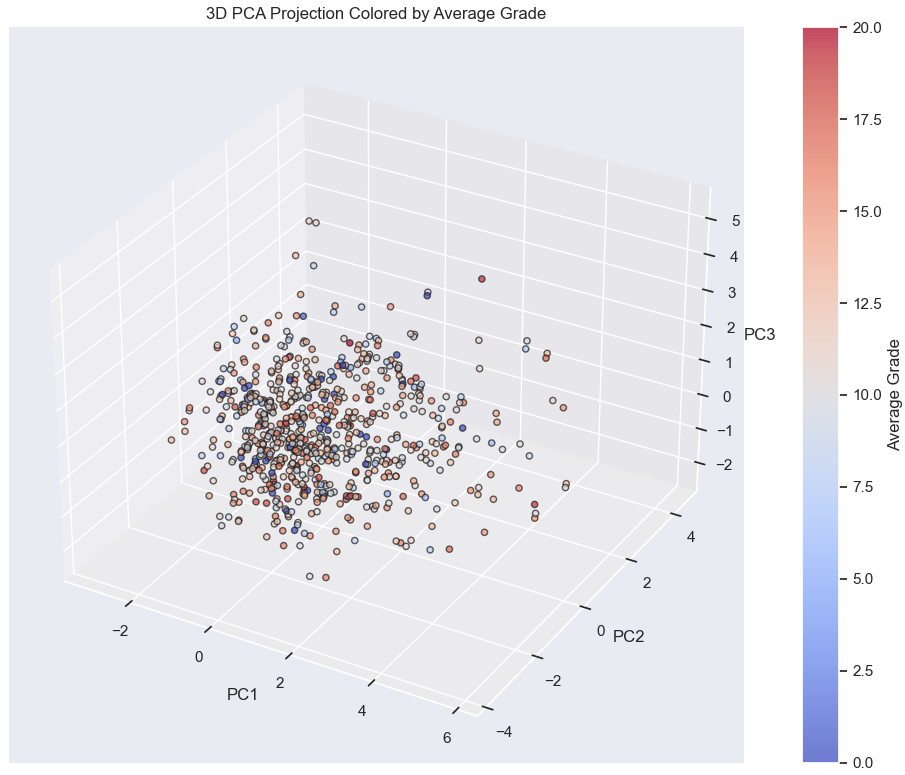
\includegraphics[scale=0.28]{PCA3PC.png}
      \caption{(b) PCA con 3 PC}
  \end{minipage}
  \caption{Visualización de los datos proyectados sobre 2 y 3 componentes principales mediante PCA.}
\end{figure}

En primer lugar, se implementó \textbf{Principal Component Analysis (PCA)} con el objetivo de estudiar la reducción de dimensionalidad y analizar los componentes principales. 
La varianza explicada por los modelos con 2 y 3 componentes principales es inferior al 30\%; no obstante, el estudio de sus loadings aporta información relevante. 
Para el 1º modelo, como cabía esperar, las variables más relevantes son \textit{T1, T2} y \textit{suspensos}, lo cual reafirma su relevancia directa en el rendimiento académico. Sin embargo, es más interesante estudiar el 2º modelo, puesto que al eliminar estas variables, las sutituyen \textit{AlcSem, AlcFin, SalAm, TiempoLib}, entre otras, que
 indican que después de las \textbf{notas}, la \textbf{vida social del estudiante} es uno de los factores más relevantes para su desempeño académico. 
 Además de estos, un tercer grupo de variables de peso que aparecen en los PC son \textit{Medu, Pedu, Relfam} y, empleando \textbf{Recursive Feature Elimination (RFE)}, 
se obtienen también \textit{Mtrab\_docencia} y \textit{Ptrab\_docencia}, lo cual pone de manifiesto que el \textbf{entorno familiar} es otro de los factores más influyentes en las notas. 

Sin embargo, PCA requiere 16 componentes para explicar el 80\% de la varianza. Al combinarlo con modelos como SVR o regresión lineal, su rendimiento disminuyó, por lo que se descartó su uso 
más allá de la exploración inicial. Este comportamiento podría deberse a la naturaleza lineal de PCA, incapaz de capturar relaciones no lineales en los datos. Por ello, se probaron 
técnicas no lineales como \textbf{ISOMAP} y \textbf{Kernel-PCA}, que operan en espacios transformados mediante distancias geodésicas o kernels y que pueden capturar relaciones más complejas entre los datos. No obstante, su combinación con modelos predictivos redujo el rendimiento entre un 20-30\%,\footnote{Exceptuando 
 Logistic Regression, dónde su combinación con Kernel-PCA lo aumentó.} 
Podemos conluir que la reducción de dimensionalidad implica la pérdida de información relevante para la predicción. Las variables no son fácilmente separables y por ello, finalmente, se empleó el \textbf{dataset completo} para el entrenamiento de los modelos.

\begin{figure}[h!]
  \centering
  \begin{minipage}[b]{0.45\textwidth}
      \centering
      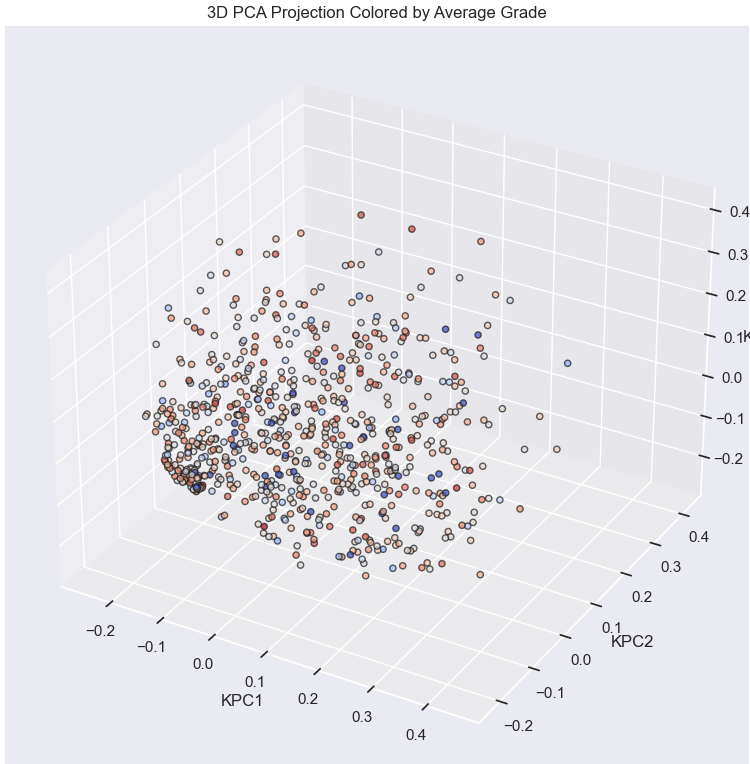
\includegraphics[scale=0.28]{KernelPCA3.png}
      \caption*{(a) Kernel-PCA con 3 PC}
  \end{minipage}
  \hfill
  \begin{minipage}[b]{0.45\textwidth}
      \centering
      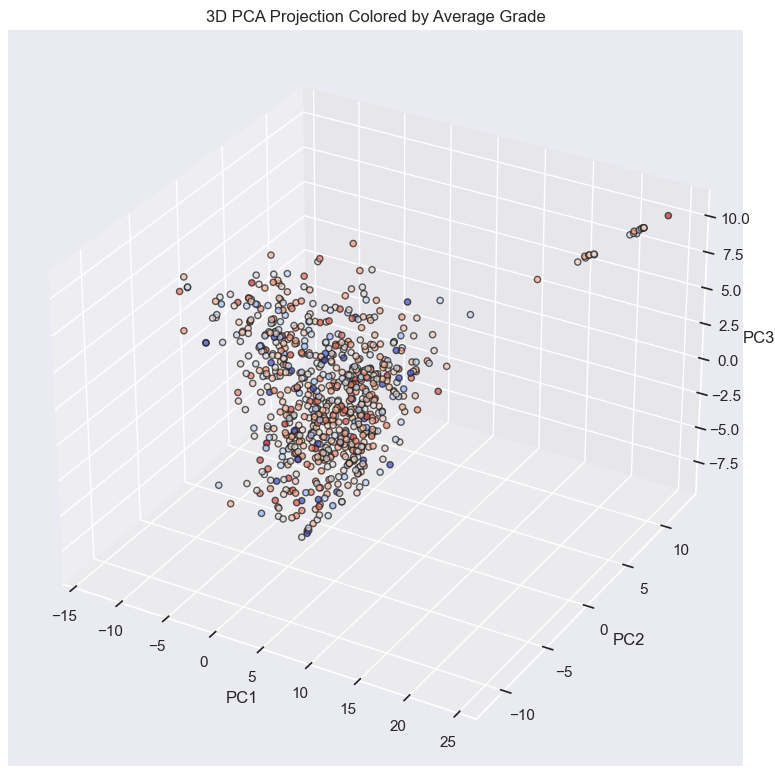
\includegraphics[scale=0.28]{ISOMAP3.png}
      \caption*{(b) ISOMAP con 3 PC}
  \end{minipage}
  \caption{Aplicación de Kernel-PCA e ISOMAP con 3 PC}
\end{figure}

Asimismo, se aplicaron técnicas de \textbf{Clustering} a los datos (combinadas con PCA). Utilizando la métrica del \textit{Elbow Method} y de la \textit{Silueta}, se obtuvo el número óptimo de clusters (2-3), que coincide con los grupos de variables relevantes identificados anteriormente. No obstante, los valores obtenidos tras aplicar K-Means (Silueta: 0.233; Índice de Davies-Bouldin: 1.341) indican una calidad media en la segmentación, reafirmando la dificultad al separar los datos. 
Experimentalmente, se probó a añadir una nueva variable a los datos indicando la pertenecia a los clusters para entrenar a un regresor lineal, pero esto no modificó su \textit{performance}, por lo que finalmente, usando la filosofía de la \textit{Navaja de Occam},
se descartó el uso activo del clustering en los modelos.

\begin{figure}[h!]
  \centering
  \begin{minipage}[b]{0.45\textwidth}
      \centering
      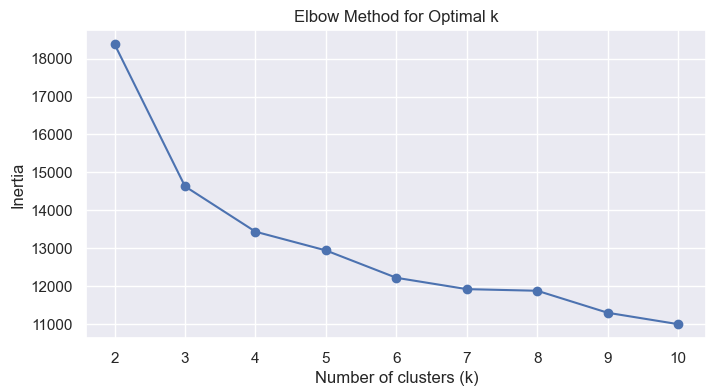
\includegraphics[scale=0.40]{Elbow_Method.png}
      \caption{(a) Elbow Method}
  \end{minipage}
  \hfill
  \begin{minipage}[b]{0.45\textwidth}
      \centering
      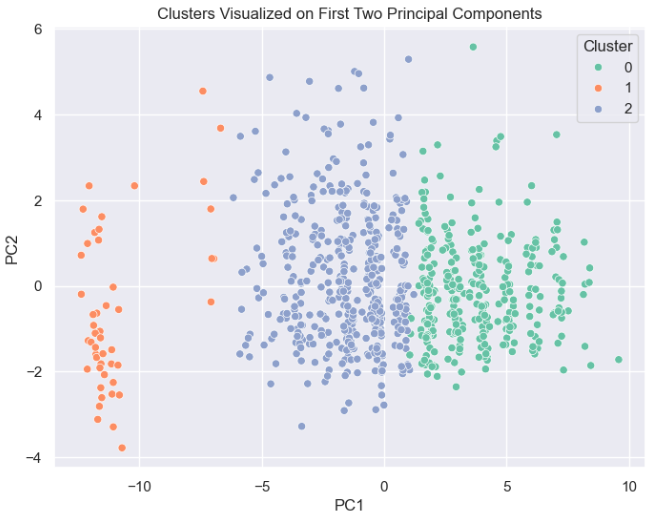
\includegraphics[scale=0.4]{Clusters.png}
      \caption{(b) Separación en clusters}
  \end{minipage}
\end{figure}

Aunque las técnicas de aprendizaje no supervisado no fueron incorporadas directamente en los modelos finales, su aplicación contribuyó significativamente a una comprensión más profunda de la estructura y relaciones entre las variables del conjunto de datos, lo cual resultó de gran valor para el desarrollo y justificación del enfoque predictivo adoptado.
La conclusión más relevante, utilizar el dataset entero sin reducir la dimensionalidad, llevó al descarte de modelos como KNNeighbours, que podían verse afectados por el \textit{curse of dimensionality}.

\subsection{Análisis adicional}


En paralelo al análisis anterior, y con el objetivo de ampliar el conocimiento sobre las variables, se utilizaron las capacidades explicativas de distintos modelos para evaluar la importancia relativa de cada característica.

Se estudió la representación conjunta de cada par de variables, empleando como código de color las distintas clases (0-20) para identificar posibles relaciones entre los datos\footnote{Ver la matriz completa en el fichero \textit{Exploratory\_Data\_Analysis}}, pero sólo se encontró un patrón claro con \textit{T1} y \textit{T2}, 
demostrando de nuevo que son variables muy significativas para la predicción.

\begin{figure}[ht]
  \centering
  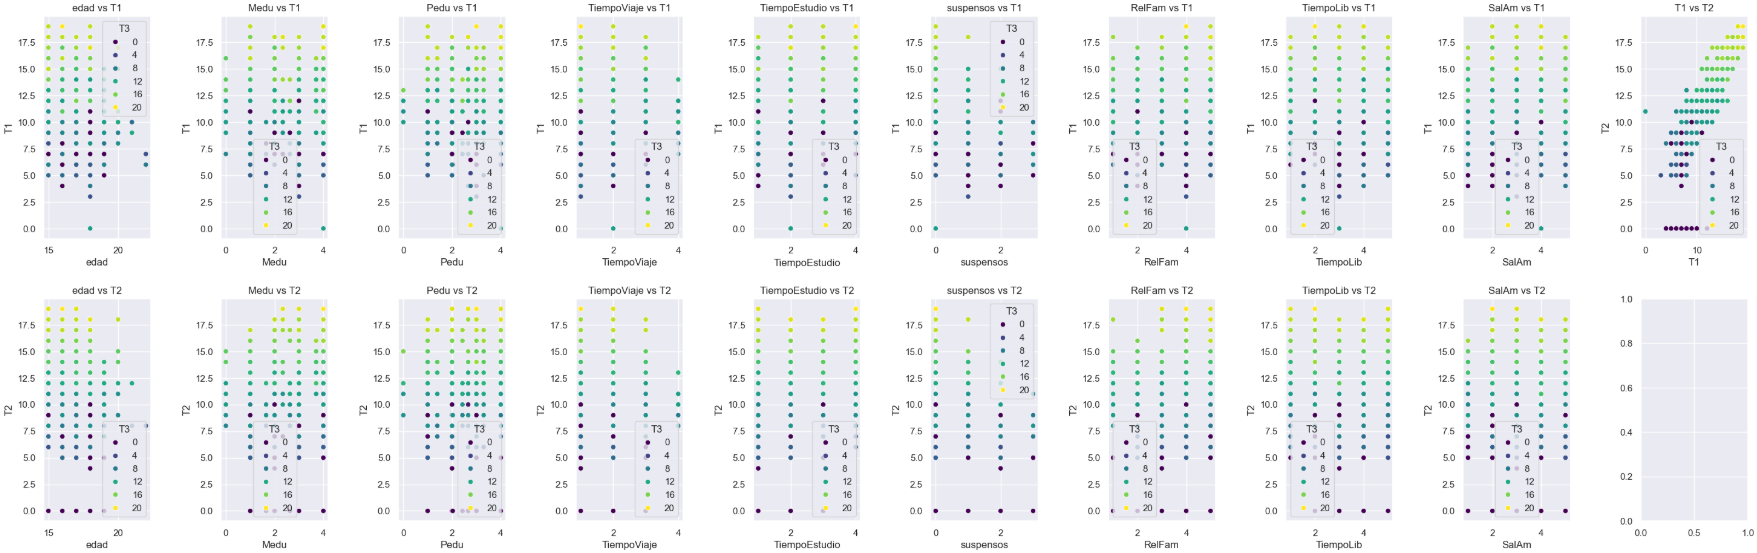
\includegraphics[width=0.9\textwidth]{Plot_Var_T1T2.png}
  \caption{Scatter Plot con T1 y T2}\label{fig:scatter}
\end{figure}

\begin{figure}[h!]
  \centering
  \begin{minipage}{0.65\textwidth}
    Uno de los algoritmos con mejor desempeño en ambos modelos, como se verá más adelante, fue \textbf{Random Forest}. 
    Vemos que las variables a las que asigna un mayor peso coinciden en su mayoría con las obtenidas con PCA y con otros métodos. Asimismo, vemos la asignación de mayor peso a algunas variables nuevas (\textit{razon\_otras, apoyo\_si}, etc.), pero esto puede depender del corte de los datos,
    ya que los árboles suelen tener una varianza alta.

    Por último, podemos ver la relevancia de T1 y T2 reflejada en que T2 tiene asignada casi la totalidad de la \textit{Feature importance}. 
    
    Cabe recalcar que T1 y T2 están muy correlacionadas (Pearson: 0.863), por lo que una asignación de pesos desequilibrada, como en este modelo, no significa que una de ellas sea significativamente más importante que la otra.
  \end{minipage}
  \hfill
  \begin{minipage}{0.3\textwidth}
      \centering
      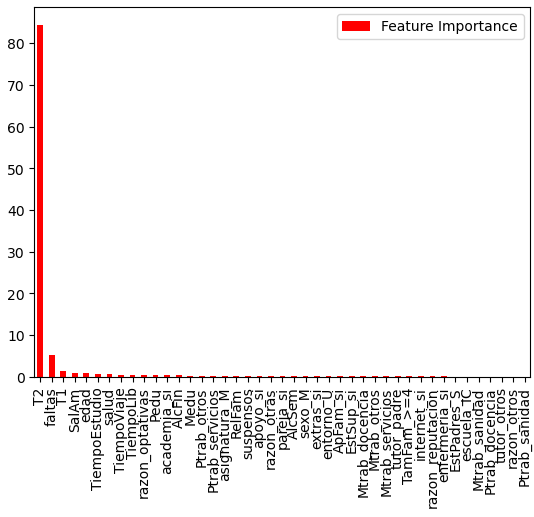
\includegraphics[width=\textwidth]{RF_var.png}
      \caption{Feature importance en Random Forest}
      \label{fig:RF}
  \end{minipage}
\end{figure}

A pesar de que el modelo de \textbf{regresión} logística no tiene el mejor rendimiento, al ser un clasificador, es interesante emplearlo, junto con regularización Lasso, para ver la evolución de los pesos de las variables para cada una de las clases, lo que aporta una mayor profundidad en el análisis.
El estudio se ha realizado sin tener en cuenta \textit{T1} y \textit{T2} y podemos ver que para las notas más bajas las variables relacionadas con la vida social y la familia son las más importantes, mientras que para las notas más altas, influyen variables más variadas.
Es interesante ver que para las notas más altas (Clase 20), muchas de las variables relacionadas con la vida social (\textit{AlcSem, AlcFin} y \textit{faltas}) se comportan de manera casi idéntica, lo que refleja un grado de relación grande, que ya hemos visto en el análisis anterior.

\begin{figure}[H]
  \centering
  \begin{minipage}[b]{0.3\textwidth}
      \centering
      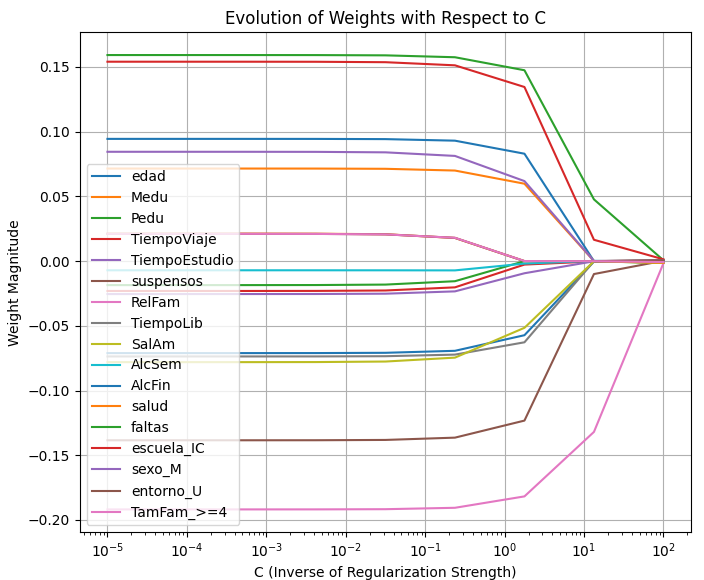
\includegraphics[scale=0.25]{FI_Class1.png}
      \caption{(a) Clase 1}
  \end{minipage}
  \hfill
  \begin{minipage}[b]{0.3\textwidth}
      \centering
      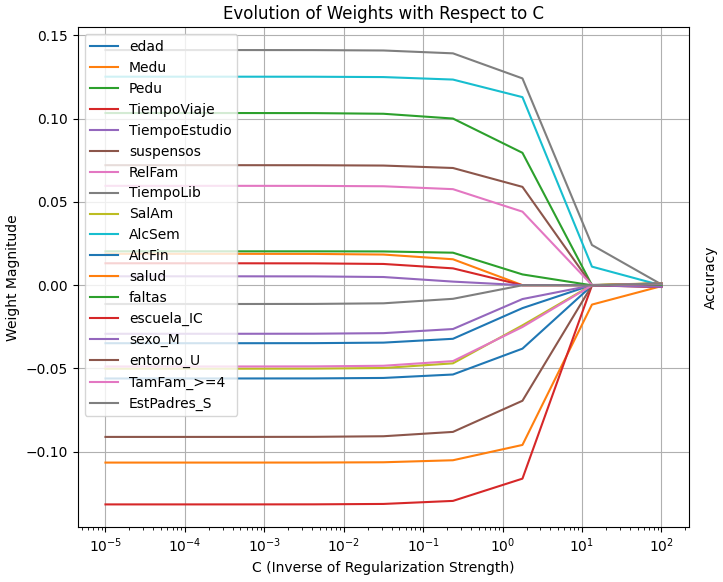
\includegraphics[scale=0.25]{FI_Class10.png}
      \caption{(b) Clase 10}
  \end{minipage}
  \hfill
  \begin{minipage}[b]{0.3\textwidth}
      \centering
      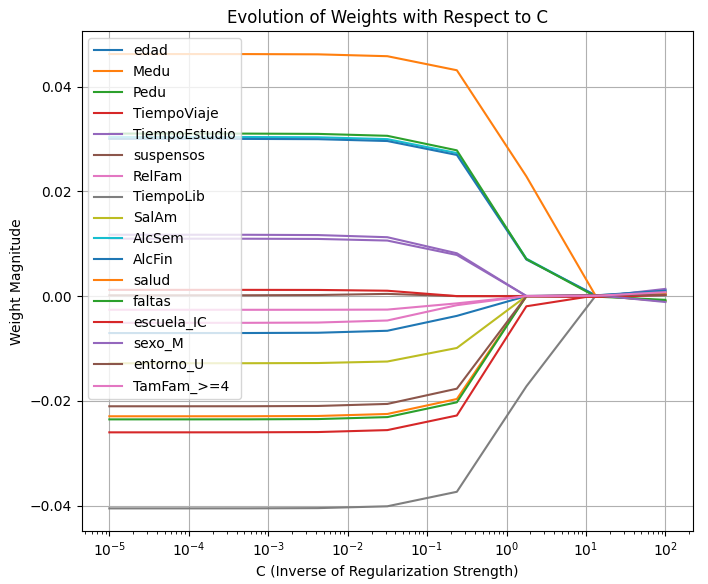
\includegraphics[scale=0.25]{FI_Class20.png}
      \caption{(c) Clase 20}
  \end{minipage}
  \caption{Feature Importance para tres clases}
\end{figure}


\section{Implementación y comparación de los dos modelos predictivos}

En esta sección se presentan los algoritmos con mayor rendimiento para ambos enfoques, junto con los criterios que justifican la elección de los modelos finales.

El desarrollo completo del análisis se encuentra en \textit{notebooks}. Las pruebas realizadas sobre los datos con los modelos iniciales se encuentran en \textit{Model1\_Testing} y \textit{Model2\_Testing}.
La selección de los parámetros de los modelos finales por validación cruzada se puede consultar en \textit{Final\_Model1\_Tuning} y \textit{Final\_Model2\_Tuning}. Por último, las métricas mostradas en el informe
se obtuvieron en \textit{Metrics\_Evaluator}.

\subsection{Análisis Técnico de los Modelos Finales}
Los modelos finales fueron todos programados manualmente.\footnote{Los códigos de los modelos pueden ser consultados en el módulo \textit{Models}.} \textbf{Linear Regression}, \textbf{Logistic Multiclass Regressor},
\textbf{Support Vector Regressor (SVR)}, \textbf{Bagging Tree Ensemble}, \textbf{Random Forest Tree Ensemble} y \textbf{Boosting Tree Ensemble}.

El propósito de este informe no es profundizar en la explicación de los modelos, por lo que me limitaré a presentar brevemente la idea principal de aquellos que no han sido abordados en clase.

\textbf{Variantes de Linear Regression:} Inicialmente, el modelo de Regresión Lineal presentó el mejor rendimiento entre las alternativas evaluadas. Con el objetivo de mejorar su desempeño, diseñé distintas variantes. Los dos modelos que lograron incrementar la \textit{performance} fueron: 


\begin{itemize}
  \item \textbf{LR\_Ensemble}: Un Ensemble de modelos de regresión lineal utilizando Random Forest como método de agregación.
  \item \textbf{LR\_Relations}: Una versión modificada que incorpora relaciones específicas identificadas en los datos (EDA). Esta variante incrementa de manera consistente los \textit{scores} de LR en varios puntos.
\end{itemize}

\textbf{Stacking Regressor:} 
Un Stacking Regressor, definido brevemente, combina múltiples modelos de regresión (\textit{estimators}) y utiliza sus predicciones como entradas para un meta modelo. 
Esto permite al meta modelo aprender cómo combinar las predicciones base para minimizar el error global.
El código diseñado crea un Stacking Regressor de dos capas, pero se pueden emplear más para realizar otras funciones, como seleccionar varibles, eliminar ruido, etc.

Los modelos que he introducido como \textit{estimators} son aquellos que han mostrado el mejor desempeño sobre el conjunto de datos (\textit{Gradient Boosting, Random Forest} y \textit{Bagging}), con los hiperparámetros optimizados por validación cruzada.

\begin{figure}[ht]
  \centering
  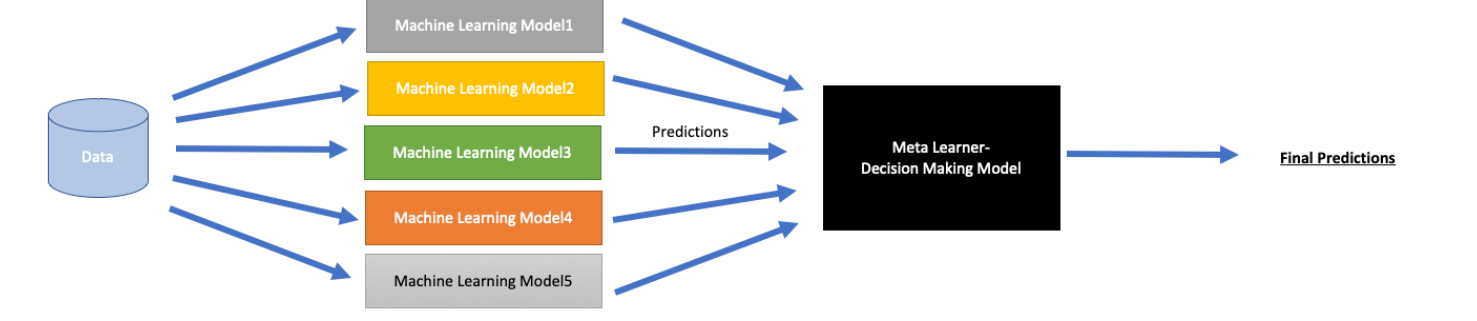
\includegraphics[width=0.7\textwidth]{Stack_Explanation.png}
  \caption{Funcionamiento del Stacking Regressor}
\end{figure}

\subsection{Modelo 1: Enfoque Predictivo con la Información Completa del Dataset}

Tras analizar múltiples modelos, se concluyó que los regresores superan consistentemente a los clasificadores, con una mejora media del 20\% en las métricas. Por ello, se descartó en una fase inicial continuar con clasificadores y se priorizó profundizar en modelos de regresión.

Los modelos de clasificación probados junto con su \textit{Accuracy} media fueron \textbf{Logistic Regression} (0.28), \textbf{Logistic Regression con Kernel-PCA} (0.57), \textbf{Support Vector Classifier (SVC)} (0.31), \textbf{Random Forest Classifier} (0.46) y  \textbf{Bagging Classifier} (0.45). 
Se programaron manualmente Logistic Regression, Random Forest Classifier y  Bagging Classifier.

La Tabla~\ref{table-M1} muestra los mejores modelos de regresión. Para garantizar la consistencia de las métricas, y evitar depender de puntuaciones obtenidas en particiones específicas del conjunto de datos, los valores presentados se corresponden con los promedios obtenidos tras entrenar más de 1200 modelos por cada técnica, utilizando datos reordenados aleatoriamente en cada iteración.

Otros modelos de regresión entrenados, junto con sus valores \textit{$R^2$} medios fueron \textbf{Support Vector Regressor (SVR) con Kernel-PCA} (0.80), \textbf{Linear Regression con ISOMAP} (0.61) y \textbf{Linear Regression con Kernel-PCA} (0.80). Todos ellos fueron descartados para el proceso de validación cruzada ya que tienen una \textit{performance} inferior.
Los modelos de árboles individuales fueron descartados a favor de los \textit{Ensembles} (TE).

\begin{table}[H]
  \caption{Modelos de regresión (Modelo 1)}
  \label{table-M1}
  \centering
  \begin{tabular}{lccccc}
    \toprule
    \multicolumn{6}{c}{Comparativa entre modelos} \\
    \cmidrule(r){1-6}
    Nombre & R² Score Test & MAE & MSE & R² Score Train & $\Delta$Score \\
    \midrule
    Linear Regression (LR)  & 0.8301 $\pm$ 0.0335 & 0.9968 & 2.6484 & 0.853 & 0.0229\\
    LR con relaciones   & 0.8338 $\pm$ 0.0327 & 1.0010 & 2.6682 & 0.854 & 0.0207 \\
    Ensemble de LR      & 0.8320 $\pm$ 0.0334 & 1.0011 & 2.6847 & 0.852 & 0.0200\\
    Stacking Regressor  & 0.8664 $\pm$ 0.0308 & \textbf{0.8890} & \textbf{2.1194} & 0.936 & 0.0696\\
    Bagging TE.         & 0.8531 $\pm$ 0.0366 & 0.9271 & 2.3367 & 0.979 & 0.1259\\
    Random Forest TE.   & 0.8552 $\pm$ 0.0343 & 0.9119 & 2.2354 & 0.980 & 0.1248\\
    Gradient Boosting TE.& \textbf{0.8682 $\pm$ 0.0304} & 0.8945 & 2.1335 & 0.926 & 0.0578\\
    SVR                 & 0.8331 $\pm$ 0.0371 & 0.9265 & 2.7643 & 0.838 & \textbf{0.0049}\\
    \bottomrule
  \end{tabular}
\end{table}

% Para \textbf{Gradient Boosting Regressor}, presente en los dos modelos con mejores resultados, ha sido muy importante la selección de parámetros, puesto que su \textit{score} era de los más variables (0.7-0.9).

% \begin{figure}[ht]
%   \centering
%   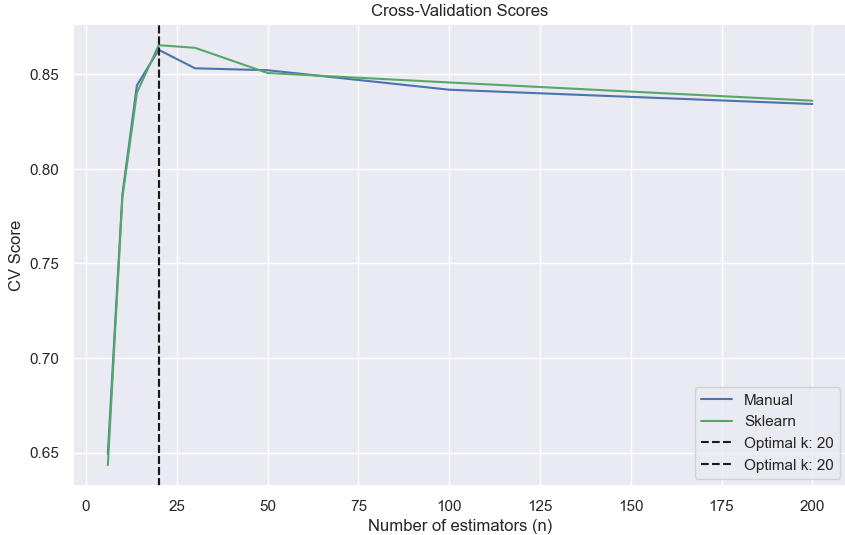
\includegraphics[width=0.3\textwidth]{CV_Boosting_N.png}
%   \caption{GBoosting score (sklearn y manual) para \textit{n\_estimators}.}
% \end{figure}

Podemos observar que \textbf{Gradient Boosting Regressor} presenta el mejor rendimiento general, mientras que \textbf{Stacking Regressor} tiene los errores más bajos. No obstante, la diferencia entre ambos modelos es inferior al 1\%, lo que indica un desempeño comparable.
Además, al contrario que Bagging y Random Forest, tienen una $\Delta$Score\footnote{$\Delta$Score = R² Score Train - R² Score Test} muy baja, lo que indica poco \textit{overfitting}. 
En base a los resultados obtenidos, se seleccionó el \textbf{Stacking Regressor} como modelo final, dado su foco hacia la minimización del error de predicción. Además, al integrar Gradient Boosting junto con otros de los modelos con mejor rendimiento individual, 
se logra mantener un R² score comparable al de estos modelos, beneficiándose al mismo tiempo de la robustez y capacidad de generalización que ofrece el enfoque de stacking.

Tras realizar un último análisis de la importancia de las variables en el modelo final usando \textit{SHAP}, podemos ver que todas las observaciones previas al entrenamiento de los modelos se han cumplido. La mayor parte de
las variables de peso están relacionadas con las \textbf{notas}, y podemos ver el efecto positivo (\textit{RelFam, salud}) o negativo (\textit{asignatura\_M, faltas}) que tienen en el target.


\begin{figure}[h!]
  \centering
  \begin{minipage}[b]{0.45\textwidth}
      \centering
      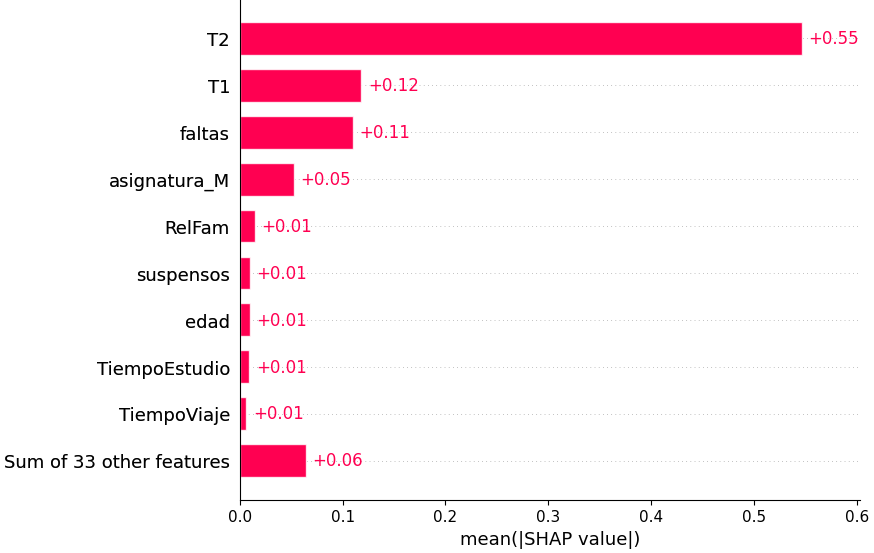
\includegraphics[scale=0.35]{Shap1_M1.png}
      \caption{(a) Feature importance}
  \end{minipage}
  \hfill
  \begin{minipage}[b]{0.45\textwidth}
      \centering
      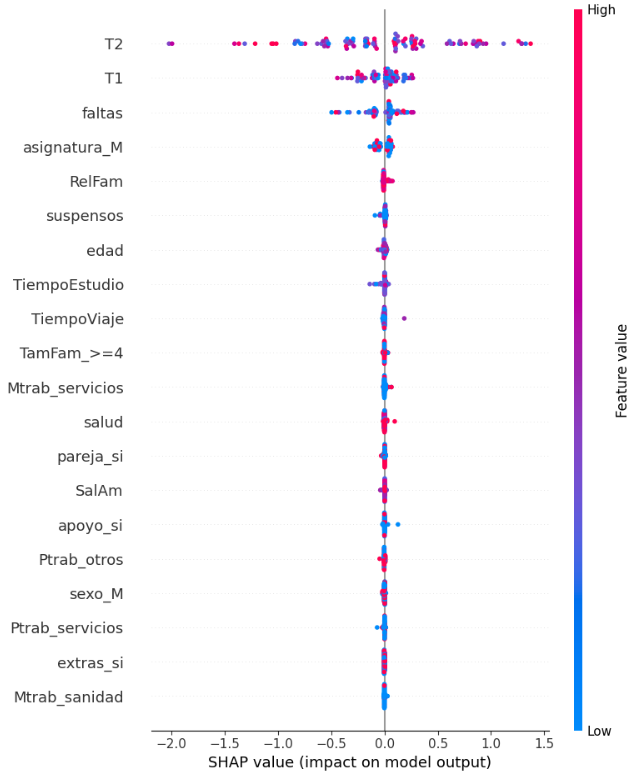
\includegraphics[scale=0.27]{Shap2_M1.png}
      \caption{(b) Gráfico Shap}
  \end{minipage}
\end{figure}


\subsection{Modelo 2: Enfoque Predictivo sin las variables T1 y T2}

Al eliminar las variables de más peso, los modelos reducen a la mitad su poder predictivo, pero se mantiene la superioridad de los regresores frente a los clasificadores.

En esta ocasión, dados los resultados anteriores, los únicos clasificadores probados, junto con su \textit{Accuracy} media fueron \textbf{Logistic Regression} (0.237) y \textbf{Classification Stack}\footnote{Usando Logistic Regression, SVC y Random Forest Classification} (0.137).
En el Modelo 1, la \textit{performance} del regresor logístico mejoró al combinarlo con \textbf{Kernel-PCA}, pero con el 2º Modelo, se ha disminuido su \textit{Accuracy} a 0.0933. Esto se debe probablemente a que los primeros componentes principales capturaban en gran medida la varianza explicada 
por las variables T1 y T2. Al eliminarlas, la estructura de varianza se ve alterada significativamente, lo que reduce la capacidad del modelo.

Adicionalmente a los regresores mostrados en la Tabla~\ref{table-M2}, se probaron a su vez \textbf{Linear Regression} (0.21), \textbf{Linear Regression con Clustering} (0.18), \textbf{Linear Regression con Kernel-PCA} (0.11) y \textbf{LR\_Relations} (0.23). Dado que 
en el modelo anterior Gradient Boosting tuvo la mejor \textit{performance}, se investigaron métodos optimizados como \textbf{CatBoosting} (0.26), \textbf{XGBoost} (0.30) y \textbf{Light GBM} (0.23). Todos estos métodos de Boosting 
están optimizados para tratar con características como datasets grandes, muchas variables categóricas o gran dimensionalidad, características que coinciden con nuestro dataset, pero tras probarlos, fueron descartados al tener una \textit{performance} inferior a Gradient Boosting.

Los resultados mostrados, al igual que con el Modelo 1, son el promedio de los resultados tras entrenar más de 900 modelos.
Podemos observar que en este caso, el \textbf{Stacking Regressor} es también el modelo con mejores resultados.

\begin{table}[H]
  \caption{Modelos de regresión (Modelo 2)}
  \label{table-M2}
  \centering
  \begin{tabular}{lccccc}
    \toprule
    \multicolumn{6}{c}{Comparativa entre modelos} \\
    \cmidrule(r){1-6}
    Nombre & R² Score Test & MAE & MSE & R² Score Train & $\Delta$Score \\
    \midrule
    Linear Regression   & 0.1999 $\pm$ 0.0625 & 2.5932 & 12.763 & 0.302 & \textbf{0.1021}\\
    Stacking Regressor  & \textbf{0.3153 $\pm$ 0.0699} & 2.4093 & \textbf{10.717} & 0.783 & 0.4677 \\
    Bagging TE.         & 0.2998 $\pm$ 0.0806 & 2.3954 & 10.971 & 0.904 & 0.6042\\
    Random Forest TE.   & 0.3056 $\pm$ 0.0768 & \textbf{2.3881} & 10.916 & 0.905 & 0.5994\\
    Gradient Boosting TE.& 0.3005 $\pm$ 0.0810 & 2.4709 & 11.025 & 0.681 & 0.3805\\
    SVR                 & 0.2856 $\pm$ 0.0657 & 2.4193 & 11.423 & 0.730 & 0.4444\\
    \bottomrule
  \end{tabular}
\end{table}

Los resultados obtenidos son muy similares a los anteriores en cuanto a la comparación de modelos. En este caso se seleccionó el \textbf{Stacking Regressor} utilizando los mismos criterios que anteriormente, robustez y \textit{performance}.
Sin embargo, este modelo no debería ser usado para realizar predicciones, puesto que no es capaz de generalizar bien. El estudio de este modelo se debería limitar al análisis de las variables
importantes en ausencia de notas previas.

Por concluir el análisis, se han usado dos gráficas \textit{SHAP} para estudiar el efecto de las variables en la predicción final. La mayoría de las variables
más relevantes coinciden con las obtenidas en el Modelo 1. Podemos estudiar el efecto positivo (\textit{EstSup\_si}) o negativo (\textit{apoyo\_si, suspensos, faltas}) que coincide con lo estudiado, sin embargo, este
análisis es menos preciso que en el Modelo 1 puesto que el modelo tiene más varianza, y los resultados de los gráficos dependen mucho del corte de los datos.


\begin{figure}[h!]
  \centering
  \begin{minipage}[b]{0.45\textwidth}
      \centering
      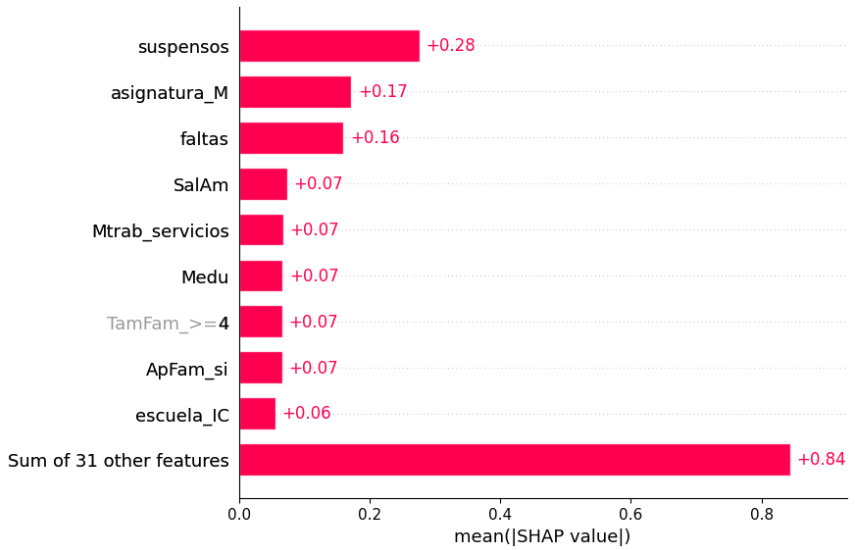
\includegraphics[scale=0.35]{Shap1_M2.png}
      \caption{(a) Feature importance}
  \end{minipage}
  \hfill
  \begin{minipage}[b]{0.45\textwidth}
      \centering
      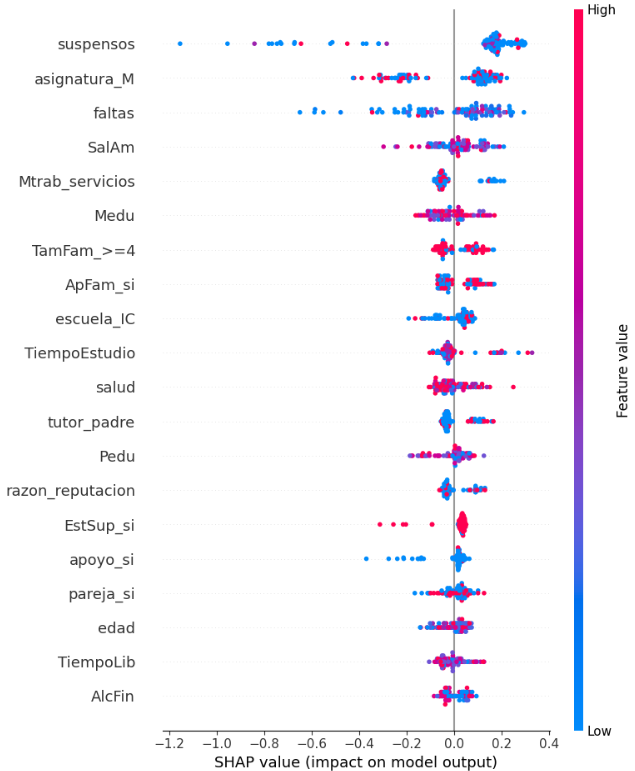
\includegraphics[scale=0.27]{Shap2_M2.png}
      \caption{(b) Gráfico Shap}
  \end{minipage}
\end{figure}



\section{Conclusiones accionables}

Para concluir, se expondrán algunas de las acciones que se pueden llevar a cabo para mejorar el rendimiento de los estudiantes en base al análisis completo del proyecto.

El análisis de los datos hecho en tres partes (EDA y conclusiones de los modelos 1 y 2) coincide en sus conlusiones consistentemente. Influyen tres grupos principales de variables a la hora de predecir el desempeño de los estudientes, los \textbf{factores académicos}, la \textbf{vida social} del estudiante, y su \textbf{entorno familiar}.
Con esta información, los centros educativos pueden enfocar sus medidas en estas áreas. 

En primer lugar, dado que los factores académicos son los más influyentes, los institutos deberían controlar una serie de métricas sobre sus estudiantes (notas, faltas, suspensos) e identificar rápidamente cualquier comportamiento que pueda empeorarlas. En caso de detectarlo, tratar de corregirlos lo antes posible.

El segundo factor más influyente es la vida social, sensibilizar al alumnado sobre la importancia de equilibrar vida social y estudio puede favorecer su rendimiento. Este tipo de medidas deberían 
aplicarse en cursos más bajos para que tengan efecto en el desarrollo de hábitos del estudiante.

Por último, el último grupo de variables importantes identificadas es entorno familiar, promover políticas de conciliación familiar podría tener un impacto positivo en sus resultados académicos. Concienciar a los padres sobre su efecto 
en la educación de sus hijos es clave. 

\section*{References}

{
\small


[1] Javier Béjar. \ \textit{Strategies and Algorithms for Clustering Large Datasets: A
Review.} \ Universidad Politécnica de Cataluña.
\url{https://upcommons.upc.edu/bitstream/handle/2117/23415/R13-11.pdf}


[2] Alfonso Cervantes Barragan. \ (2024). \ \textit{Interpreting and Validating Clustering Results with K-Means}. 
\ Medium. 
\url{https://medium.com/@a.cervantes2012/interpreting-and-validating-clustering-results-with-k-means-e98227183a4d}


[3] Connie Zhou.\ (2023). \ \textit{Unraveling Data Patterns with Isomap: A Guide to Dimensionality Reduction — Part 4}.
\url{https://medium.com/@conniezhou678/unraveling-data-patterns-with-isomap-a-guide-to-dimensionality-reduction-part-4-1d774eee69a5}

[4] (2025). \ \textit{Gradient Boosting in ML}. \ Geeks for Geeks.
\url{https://www.geeksforgeeks.org/ml-gradient-boosting/}

[5] Casper Hansen. \ (2020). \ \textit{Stack machine learning models: Get better results}. \ IBM Developers.
\url{https://developer.ibm.com/articles/stack-machine-learning-models-get-better-results/}

}

%%%%%%%%%%%%%%%%%%%%%%%%%%%%%%%%%%%%%%%%%%%%%%%%%%%%%%%%%%%%


\end{document}